\section{Experiments}
\label{sec:exp}

\subsection{Dataset}

We use a similar approach to \citet{wang2023towards} to download videos. The dataset contains 27,775 sentences(more than 20 hours) from 13,143 dog related videos.

%\subsection{Evaluation}
%We provide two different evaluations to evaluate the results in two areas, phoneme and lexical. They are complementary and evaluate the phoneme and lexical of dog vocalization understanding.
% \MY{Add a para to say that we provide two different evaluations, which are complementary and evaluating different aspects on dog vocalization understanding.}
% \KZ{Need to get the terminalogy straight in the method section.
% Don't say 5 consecutive labels, u can say phones of at least 5 frames long.
% Define ``frame'' first in the method section.}
\subsection{Phoneme Evaluation}

\paragraph{Evaluation Protocol}

A successfully classified phone should possess the following two properties: 1) phones with the same label (phoneme) should sound very similarly; 
and 2) phones with different labels are sounds that are clearly distinct. 
To verify the reliability of the dog vocalization phonemes obtained in 
\secref{sec:method}, we design a phoneme comparison experiment.
The dog vocalization sentences in the test dataset were processed using 
the operations described in \secref{sec:method} to obtain phoneme label 
sequences. Each type of label was randomly sampled and intercepted. 
To improve the accuracy of the identification by human beings, 
we intercepted phones of at least 5 frames
(with a length greater than 0.1 seconds) as samples for the accuracy test. The frames are from HuBERT(about 20ms a frame). 


\paragraph{Annotator Demographics}

The testers are two college students majoring in engineering who love small animals and participated in the experiment as volunteers.

The testers will listen to several pairs of audio segments, including segments with the same label and segments with different labels. The testers are required to use their prior knowledge to judge whether the pair of audio segments belongs to the same category.

\begin{table}
\centering
\small
\begin{tabular}{lll}
\hline
\textbf{Type} & \textbf{Labels}\\
\hline
\verb|Dog| & 1, 7, 9, 10, 11, 12, 14, 16, 17, 20-24, 26-34, \\
& 37, 40-44, 46-50 \\
\verb|Noise| & 2, 3, 4, 5, 6, 8, 13, 15, 18, 19, 25, 35, 36, \\
& 38, 39, 45 \\\hline
\end{tabular}
\caption{Dog phonemes vs noice phonemes}
\label{tab:phoneclassification}
\end{table}

\paragraph{Metrics}

In the first round of testing, two testers randomly selected 30 labels from all labels and randomly sampled 8 pairs of identical audio segments and 7 pairs of different audio segments in each label, for a total of 225 pairs of audio segments. The accuracy is shown in \tabref{tab:phonetestresult}.

During the test, we found that almost $1/3$ of the labels corresponded to noise segments. To this end, two testers conducted a noise-dog sound discrimination experiment on all 50 labels. The experiment randomly selected 5 samples from all 51 labels. The two testers first judged whether the segment was noise from the sound features. If it was impossible to judge from the audio features alone, the testers would refer to the corresponding video for judgment. The judgment results of the two testers are shown in \tabref{tab:phoneclassification}.

In order to ensure the accuracy of the consistency test of dog sound labels, after excluding noise labels, we finally sampled 30 phoneme labels randomly in dog vocalization labels. Each label has 10 test groups, including five identical label pairs and five different label pairs, for a total of 300 pairs of audio segments. The accuracy is shown in \tabref{tab:phonetestresult}.

\begin{figure}[th]
\scalebox{0.1}{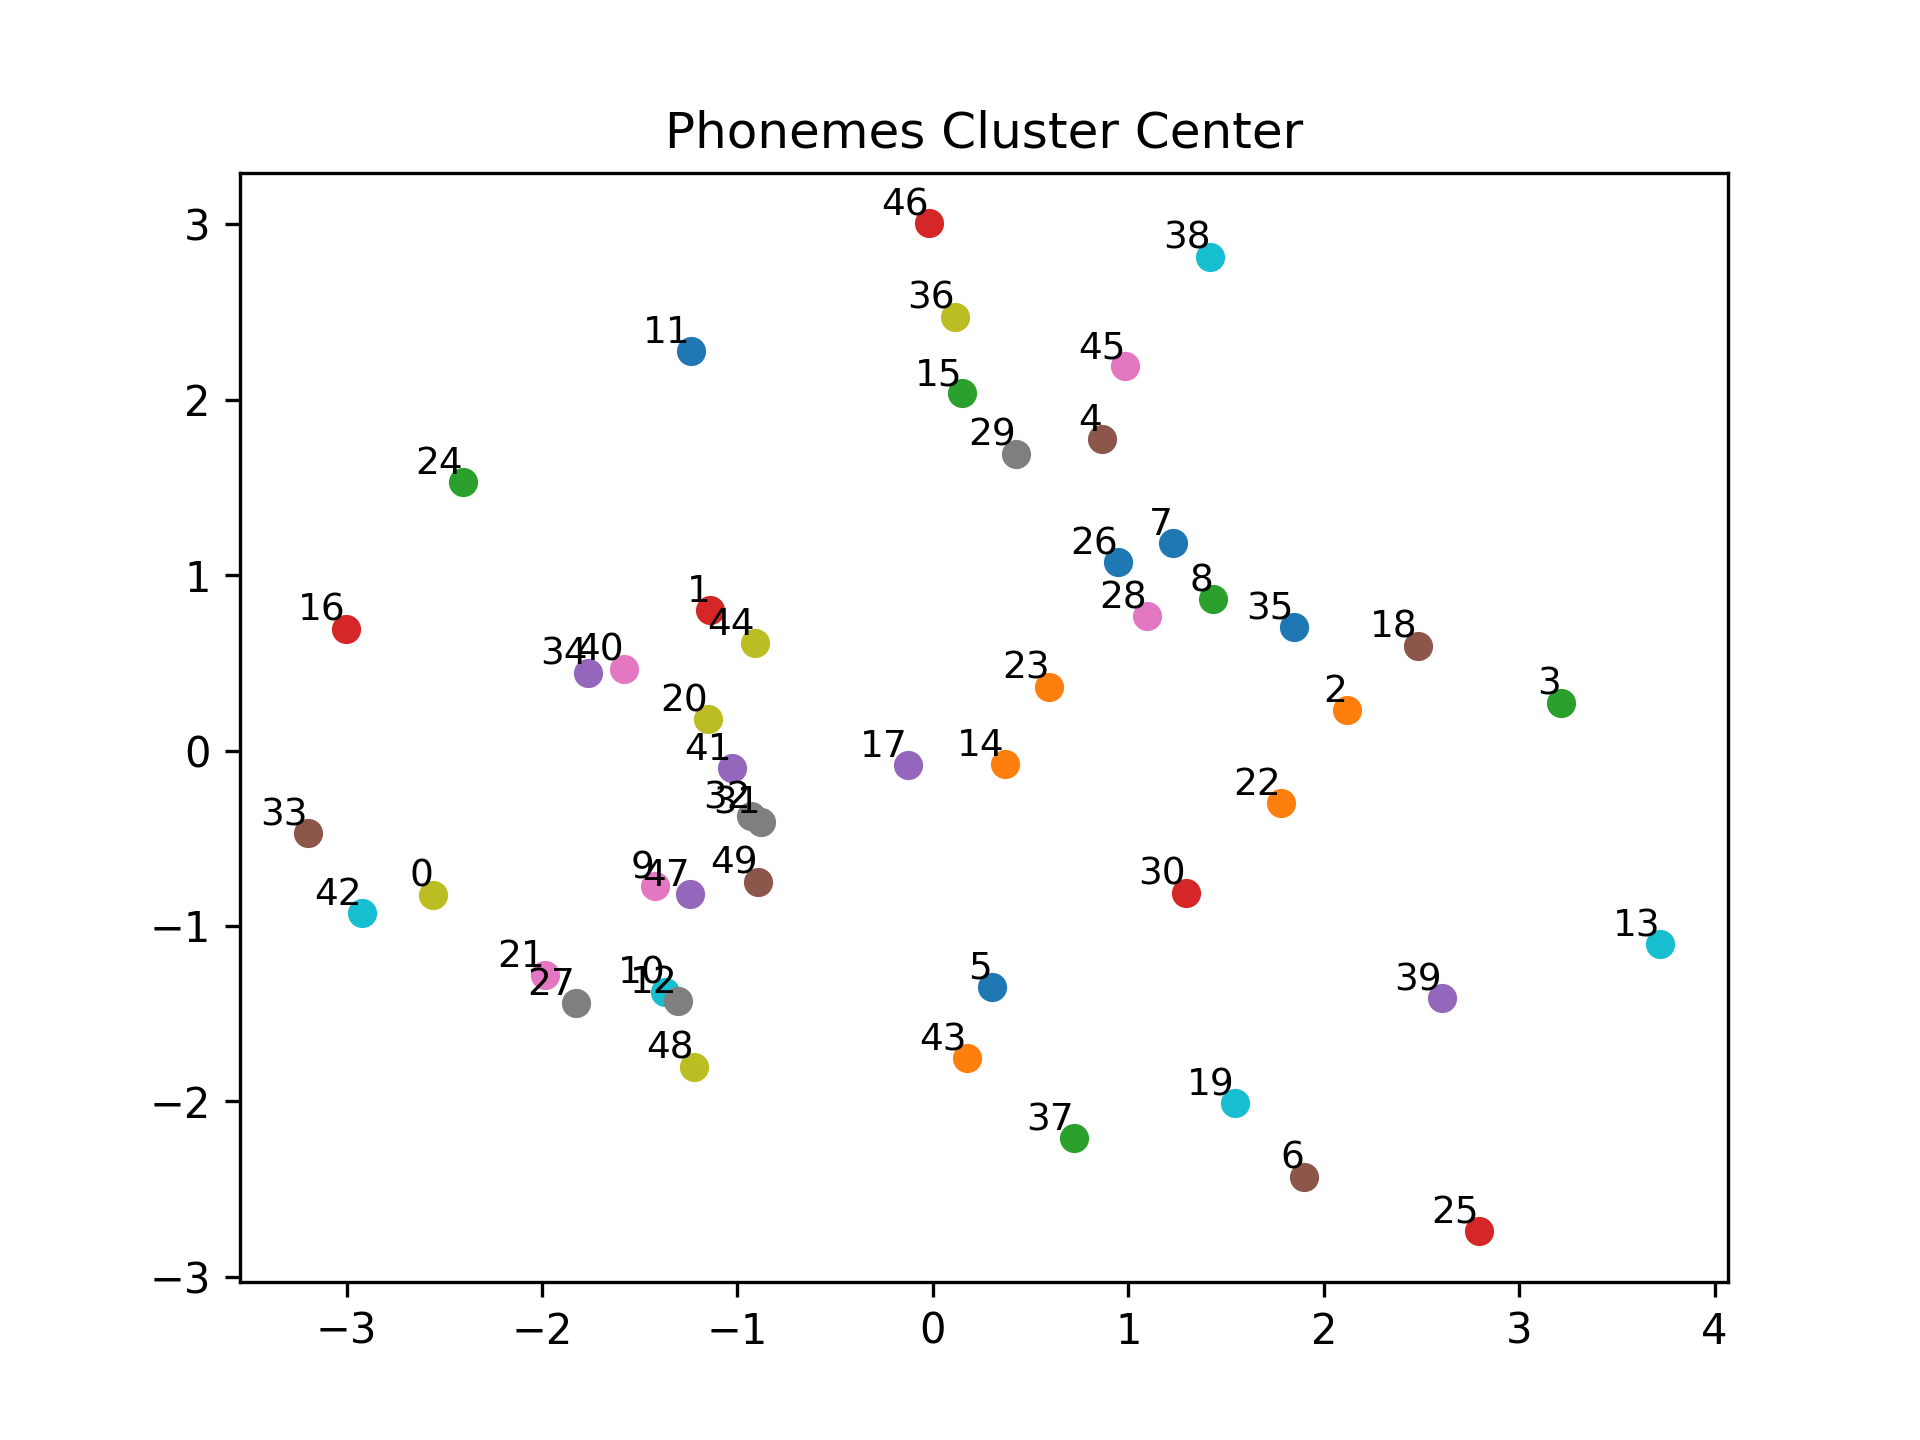
\includegraphics{phoneclustercenter.png}}
\caption{2-D Visualization of 50 phonemes from HuBERT.}
\label{fig:cluster}
\end{figure}

From the test results, we can find that the test results containing only dog sound labels are better than the test data containing noise. At the same time, the testers' judgments on the consistency of the sound are relatively consistent, and the agreement rate is above 80\% on the individual dog labels. According to the feedback from the testers, due to the large number of noise segment types, different types of noise are often classified into the same label within a limited number of labels. The clustering center point results of the audio vector representation of the 50 labels are shown in \figref{fig:cluster}. Due to the model's focus on the context based on transform, noise labels often exist around the dog sound labels, making it difficult for testers to distinguish.

%\MY{Shall we have a comparison with the phoneme labelling results from Jieyi? to show that our method can output better results with higher human agreement}

% \begin{table}[th]
% \centering
% \begin{tabular}{lc}
% \hline
% \textbf{Tester} & \textbf{Accuracy}\\
% \hline
% \verb|Tester 1| & 70\% \\
% \verb|Tester 2| & 68.3\% \\
% \verb|Tester 3| & unknown \\ 
% \verb|Agreement| & unknown \\\hline
% \end{tabular}
% \caption{Coincidence and agreement result on testing the reliability of phonemes discovery}
% \label{tab:phonetestresult}
% \end{table}


\begin{table}[th]
\centering
\small
\begin{tabular}{lcc}
\hline
\textbf{Tester} & \textbf{dog voice label} & \textbf{total label}\\
\hline
\verb|Tester 1| & 72.0 & 66.67 \\
\verb|Tester 2| & 70.5 & 64.89 \\
% \verb|Tester 3| & AudioSep & \pmb{0.7755} \\
\verb|Agreement| & 80.5 & 74.22 \\\hline
\end{tabular}
\caption{Accuracy and agreement result on testing the reliability of phonemes discovery}
\label{tab:phonetestresult}
\end{table}


%Three testers labeled the randomly sampled audio pairs. If the tester considered the audio pair to have the same label, it was marked as 1. If the tester considered the audio pair to have different labels, it was marked as 0. The consistency rate between the model and testers and agreement rate of the three testers' results with the dog vocalization transcription results are shown in \tabref{tab:phonetestresult}.
%\KZ{What do u mean by coincidence? Need to define how you compute these.}\SN{If testers give the ground truth, then we can use accuracy}

%\SN{I will modify this paragraph after get new results}We can see that the coincidence rate of the testers' judgments with the labels we obtained is around 70\%. According to the testers' feedback, about 1/3 of the test samples contained noise, which came from the dog vocalization sentences in the dataset, the judgments result is in Table \ref{tab:phoneclassification}. Due to the wide variety of noise types, several types of noise were classified as the same phoneme by the same label, which made it difficult for the testers to distinguish between noise with the same label and noise with different labels. 
%\KZ{At this point you wanna show a picture of clustering of those noisy labels
%together in the HuBERT embedding space. To back up your claim that those
%are actually noises.} 
Overall, the phoneme labels obtained are consistent with the phonemes, 
and their classification is relatively accurate. This provides us with the 
possibility to further explore how to obtain lexical discoveries of 
dog vocalizations.
%TODO add length mean, variance



\subsection{Lexical Evaluation}

\paragraph{Evaluation Protocol}

After the combination algorithm we mentioned in \secref{sec:method}, the dog vocalization sentence will be transcribed into a list composed of phoneme labels. Will it contain combinations of labels with fixed patterns, such as words? 
As one of the constituent elements of language, words should have the 
two characteristics of 1) frequently appearing in voice samples and 2) being 
able to be uttered by many different individuals. 
%\KZ{The above should have been mentioned in the method section already.
%No need to repeat it here.} 
To obtain such a ``vocabulary'', we followed the two basic characteristics of words and obtained a vocabulary composed of bigrams, trigrams, and up to six grams, according to the process described in \secref{sec:method}.
% \KZ{No need to keep repeating/mentioning sec 2!}

\begin{figure*}[h]
\centering
\scalebox{0.3}{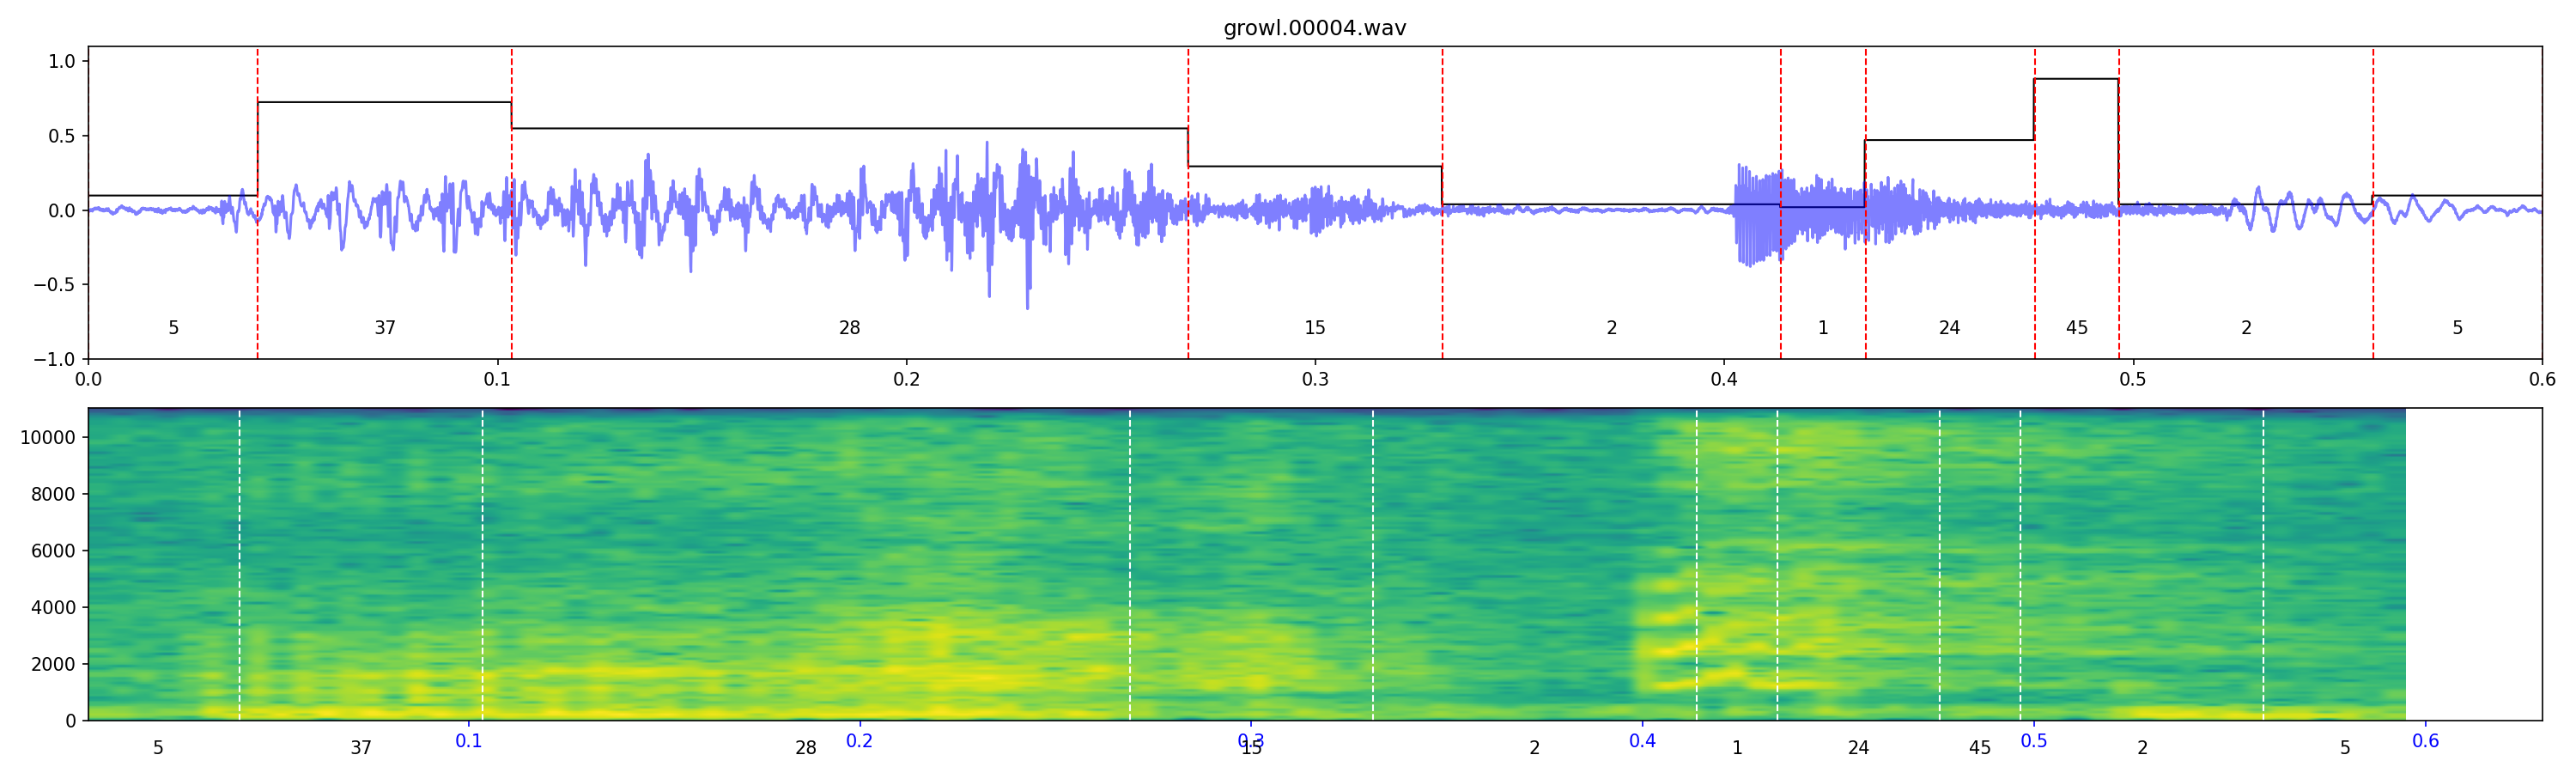
\includegraphics{growl00004hubert109.pdf}}
\caption{Segmentation and Phoneme Labelling Result of A Growl Sound. }
\label{fig:cwc}
\end{figure*}

\begin{figure}[th]
\centering
\scalebox{0.3}{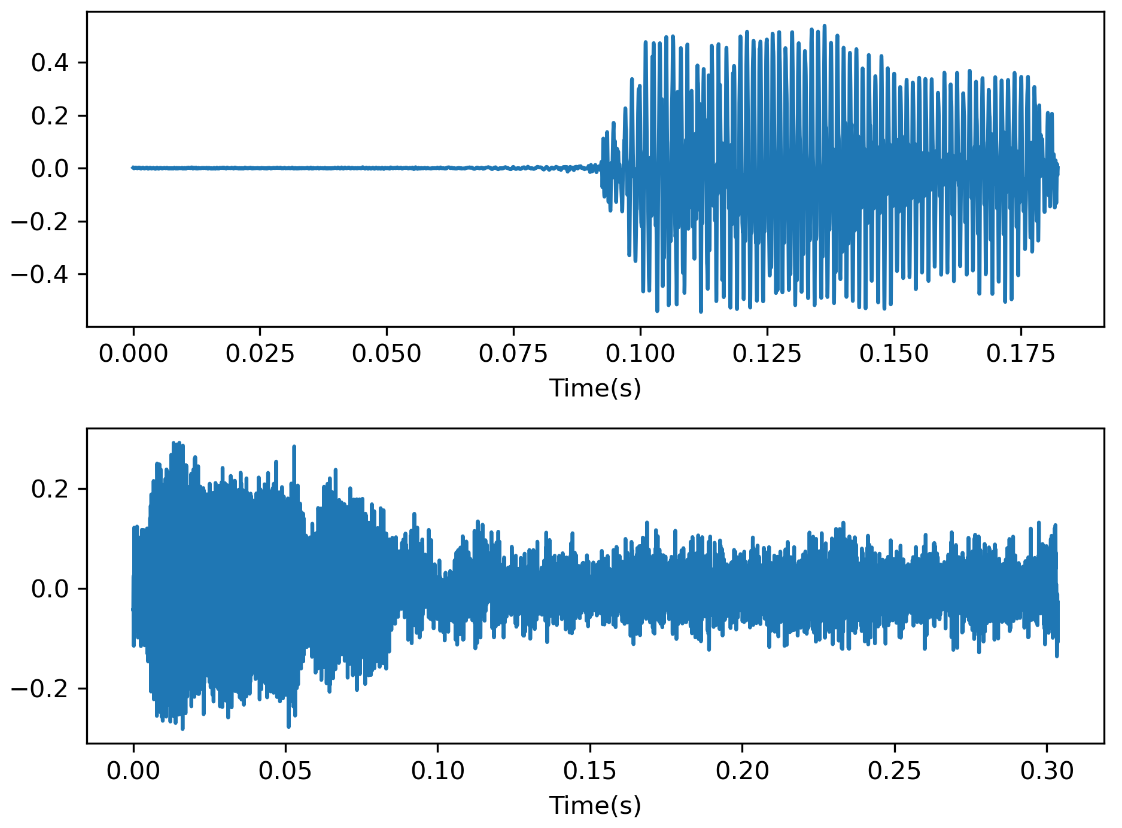
\includegraphics{full_no.jpg}}
\caption{Top: waveform of word (18, 35, 40, 33); Bottom: waveform of word (24, 26)}
\label{fig:full}
\end{figure}

Due to the accuracy of the phoneme classification labels, we shift our attention from the consistency of audio segments in the same ngram to the integrity of words in the ``vocabulary''. A word usually contains only one continuous sound, which can be reflected in the energy diagram of the audio. As shown in Figure \ref{fig:full}, whether it is based on the characteristics of the audio or from the observation angle of the energy diagram, we believe that the audio at the top is a complete pronunciation, while the audio at the bottom is not. 

In addition to measuring whether an ngram is a complete word and whether the same ngram has acoustic consistency, we also need to determine that the words in the ``vocabulary'' have a certain degree of universality, i.e., they are contained in a wide range of individual voices. 

%\begin{table}
%\centering
%\begin{tabular}{lc}
%\hline
%\textbf{Tester} & \textbf{Accuracy}\\
%\hline
%\verb|Tester 1| & 100 \\
%\verb|Tester 2| & 95 \\
%\verb|Tester 3| & unknown \\ 
%\verb|Agreement| & unknown \\\hline
%\end{tabular}
%\caption{Result of complete word score}
%\label{tab:wordcomplete}
%\end{table}

\paragraph{Metrics}

% \KZ{Don't say hire! Just say three testers did blah blah...} \SN{Done}
Two testers score 100 randomly selected samples from the ``vocabulary'', with 1 points indicating that the sample is a complete word, 0 points indicating that the sample is not a complete word. The test results is 67\%. Inevitably, due to the shorter length of Bigram, there are more of them under the same threshold; from the feedback of the testers, although some Bigram is represented as the nasal sound of a dog, there are still some incomplete audio. We speculate that this is mainly because the universality of this segment is stronger, and there are many kinds of phonemes that can be matched before and after, which leads to its higher $\delta$ value, thus increasing the value of its popularity score.%TODO analysis the result of precision

To measure the recall of the ``vocabulary'', we design two metrics, phoneme coverage and phone coverage to evaluate whether the ``vocabulary'' is universal. Phoneme coverage refers to the percentage of the number of phonemes from all words in the ``vocabulary'' to the total number of phonemes in all sentences; phone coverage refers to the percentage of the total audio duration of all words from the vocabulary to the total audio duration of all sentences.% The results of these two metrics is shown in Table \ref{tab:wordcoverage}.

\begin{figure}[th]
    \centering
    \scalebox{0.1}{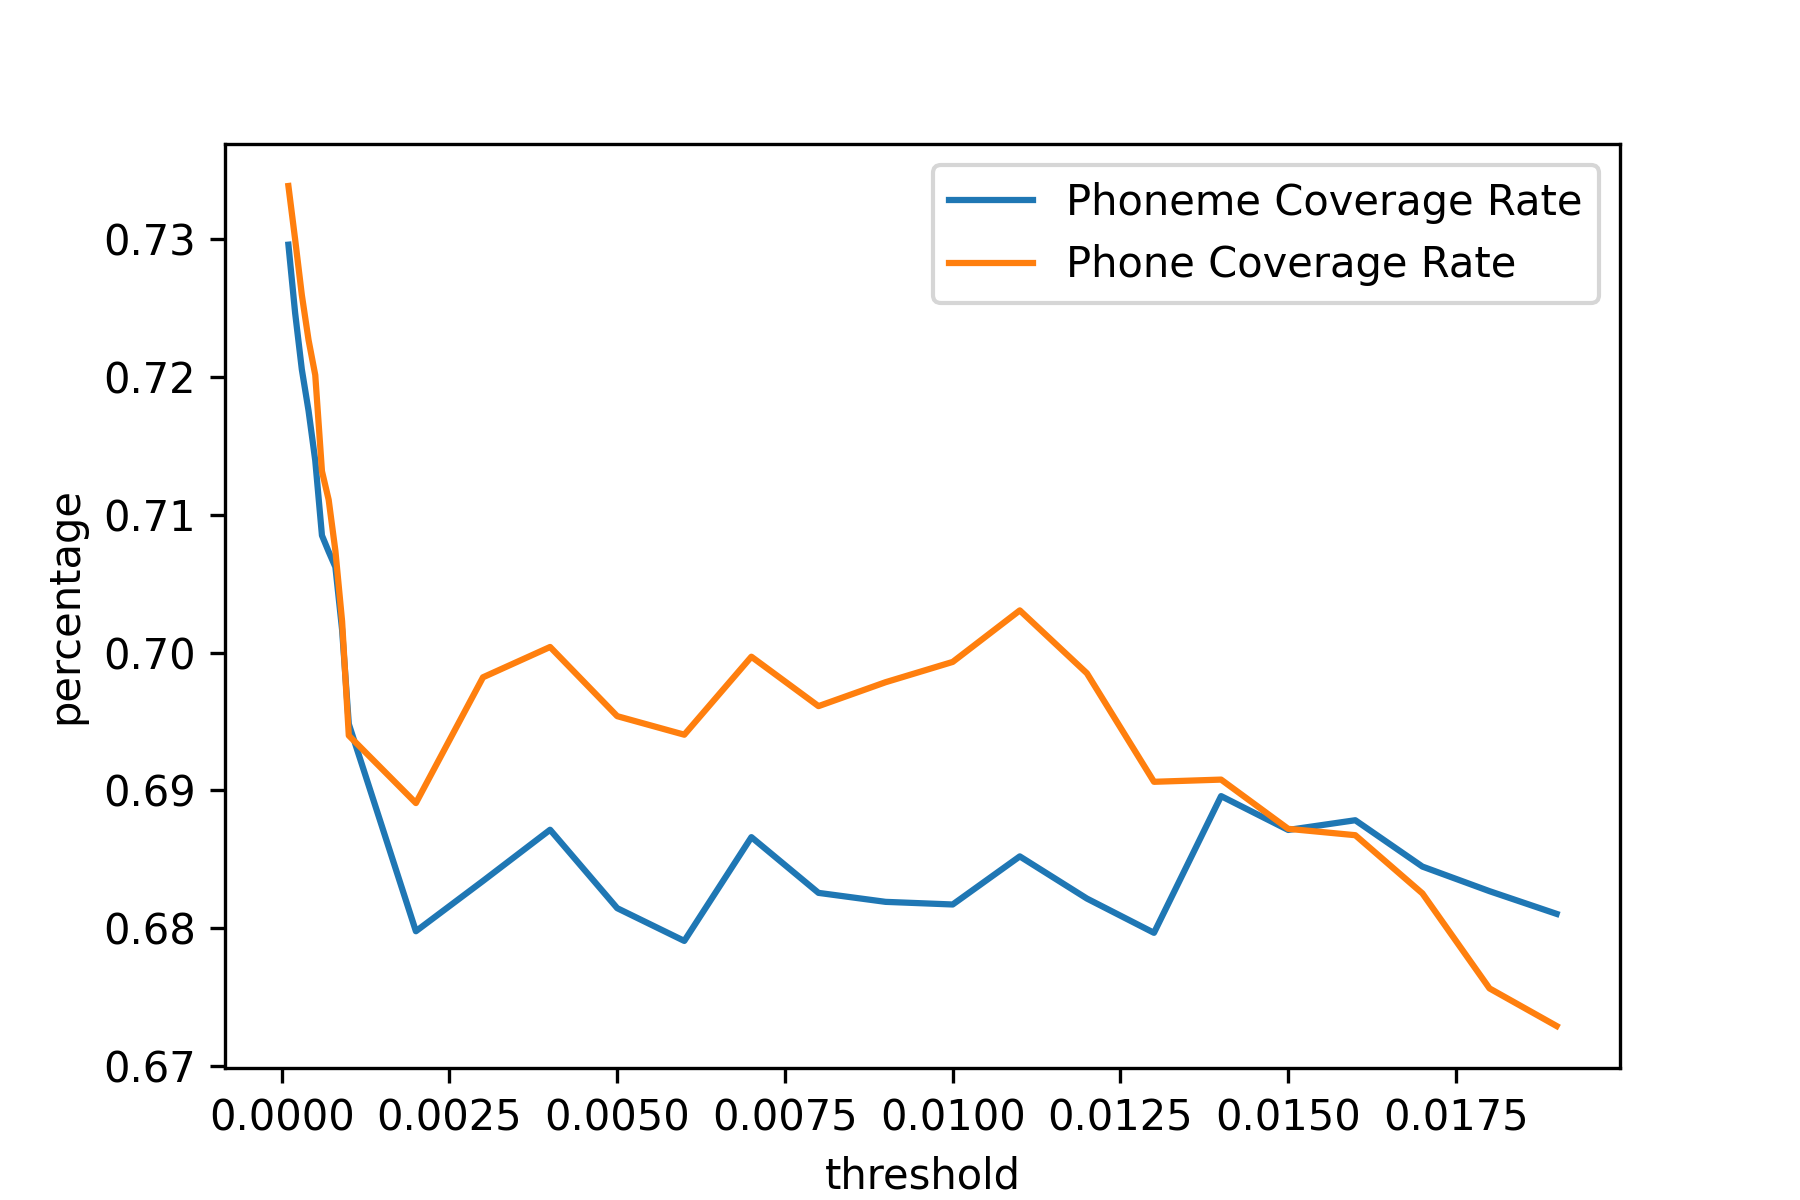
\includegraphics{wordrecall.png}}
    \caption{Phoneme Coverage and Phone Coverage on different threshold}
    \label{fig:wdc}
\end{figure}

From another perspectives, these two metrics can also help us determine the value of the threshold used to divide the ``vocabulary''. The lower the threshold value, the more words in the vocabulary, and these additional words in the vocabulary, and these additional words may also have their own meanings. However, in this work, we want to ensure that each word in the ``vocabulary'' has the highest probability of having a meaning on the basis of ensuring macro word coverage. The coverage rate results for different thresholds are shown in Figure \ref{fig:wdc}.

%TODO analysis the figure
